\section{Wireless and Mobile Networks}


\subsection{Introduction}


\subsection{Wireless Links Characteristics}

\key{Wireless Link Characteristics}
\begin{figure}[H]
  \centering
  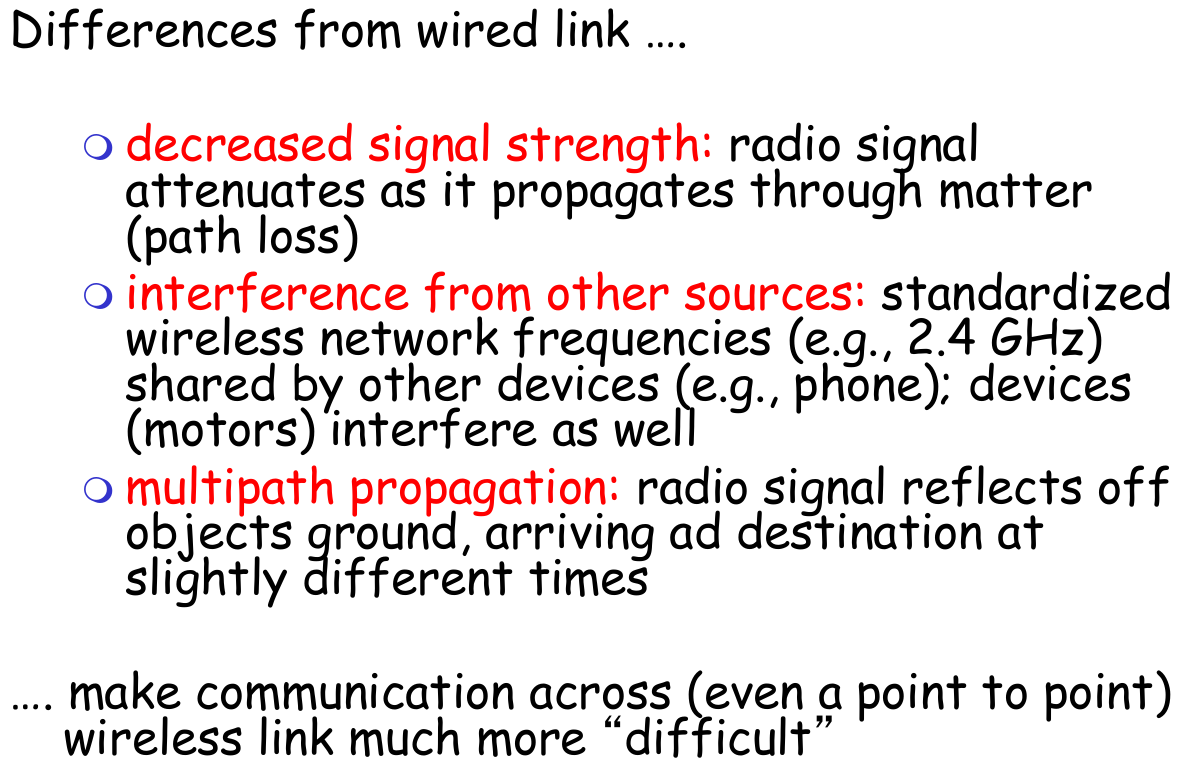
\includegraphics[width=0.48\textwidth]{wireless_char}
  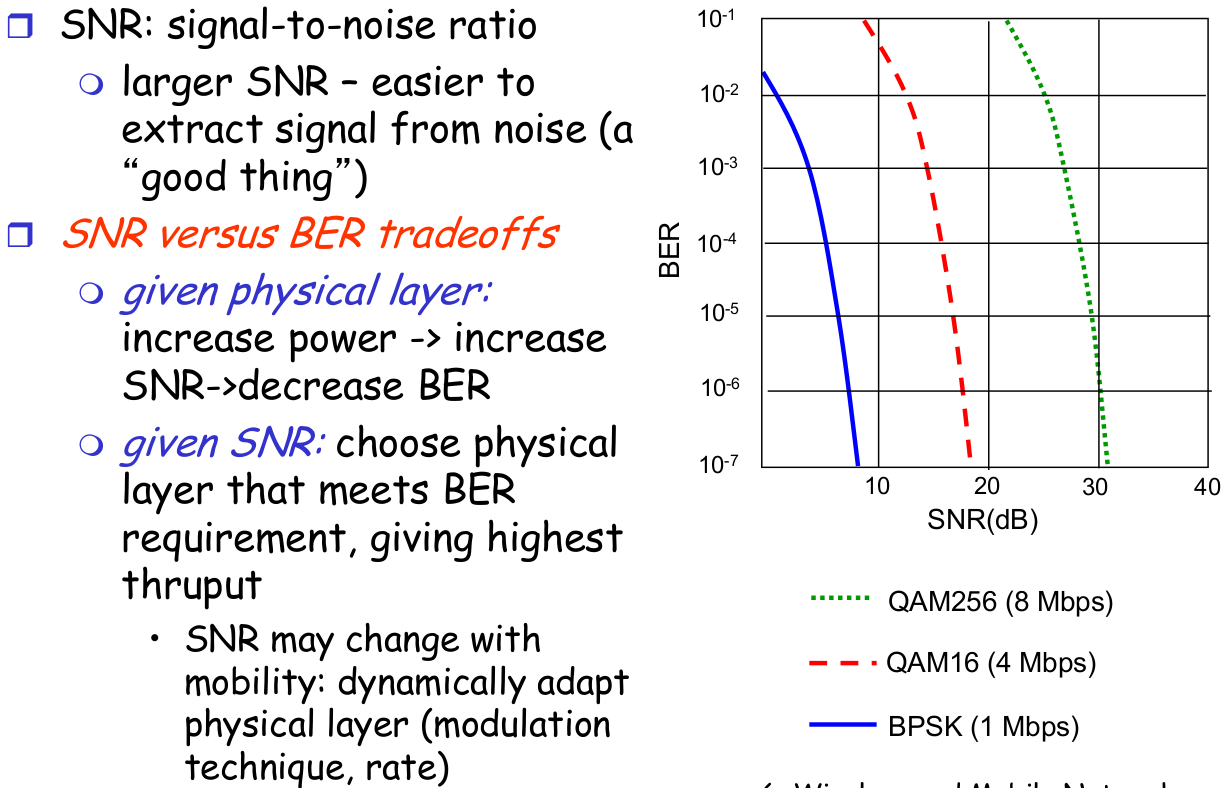
\includegraphics[width=0.48\textwidth]{wireless_char2}
\end{figure}

\subsection{IEEE 802.11 Wireless LANs (wifi)}

\key{IEEE 802.11: Multiple Access}
\begin{figure}[H]
  \centering
  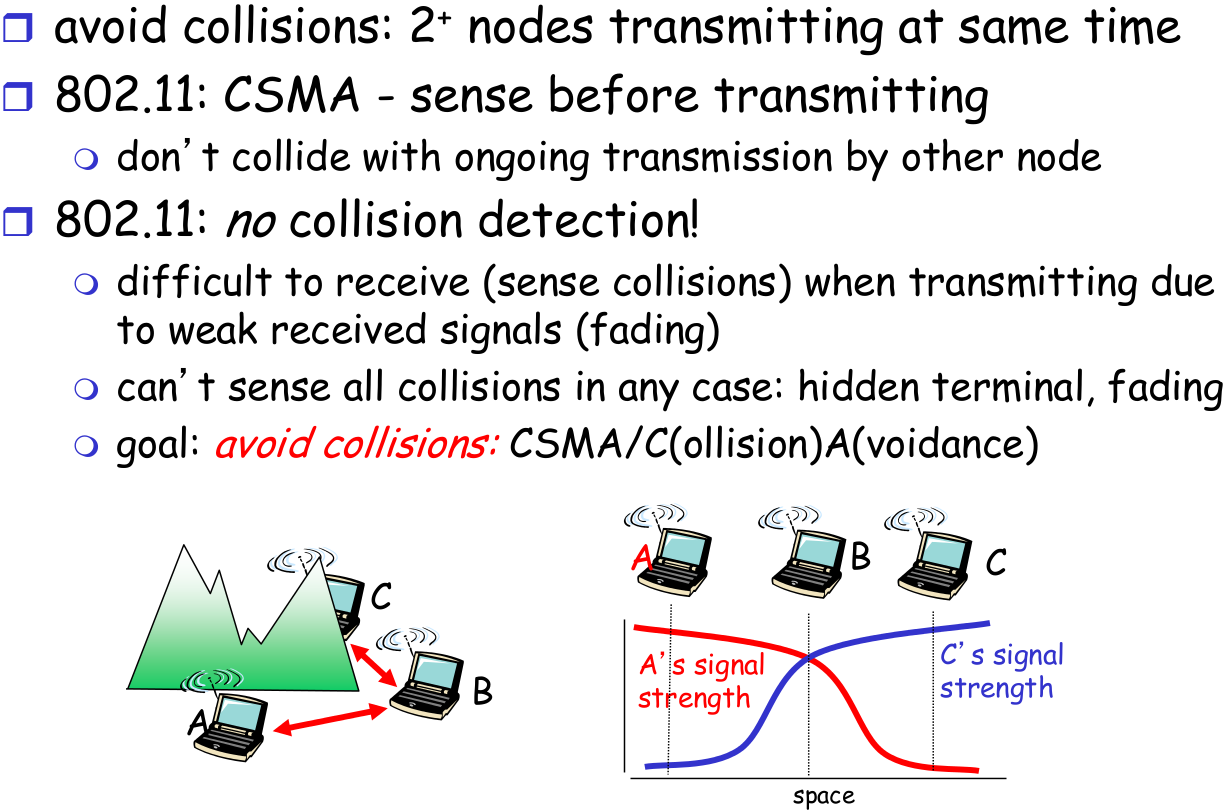
\includegraphics[width=0.48\textwidth]{csma_ca1}
\end{figure}

\key{Collision Avoidance: RTS-CTS exchange}
\begin{figure}[H]
  \centering
  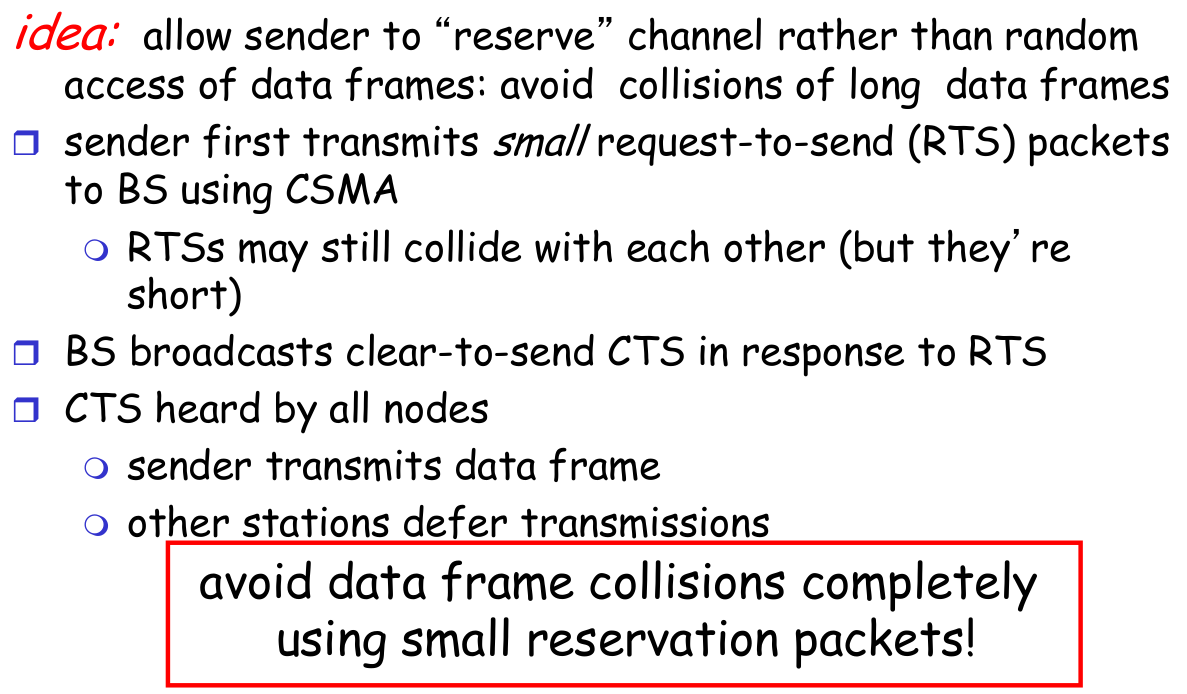
\includegraphics[width=0.48\textwidth]{rts_cts1}
  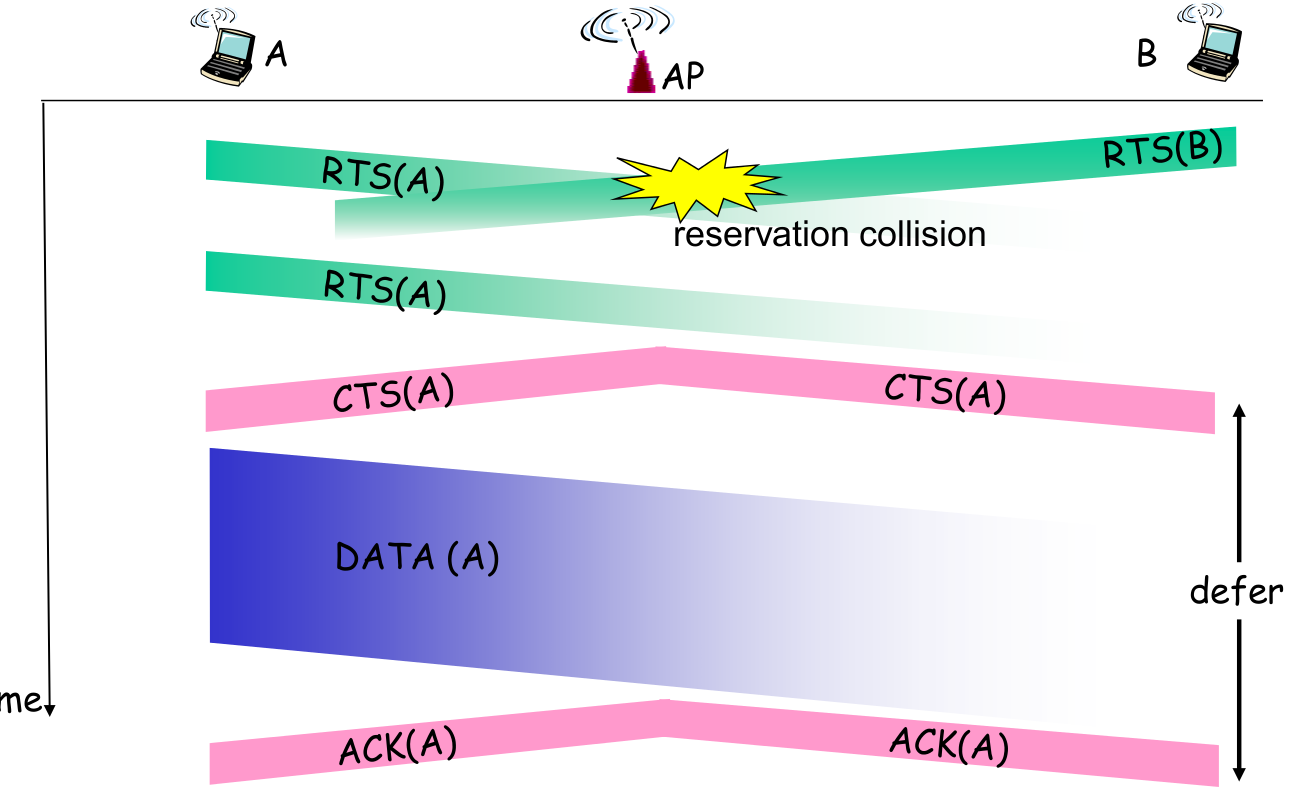
\includegraphics[width=0.48\textwidth]{rts_cts2}
\end{figure}

\key{802.11 frame: addressing}
\begin{figure}[H]
  \centering
  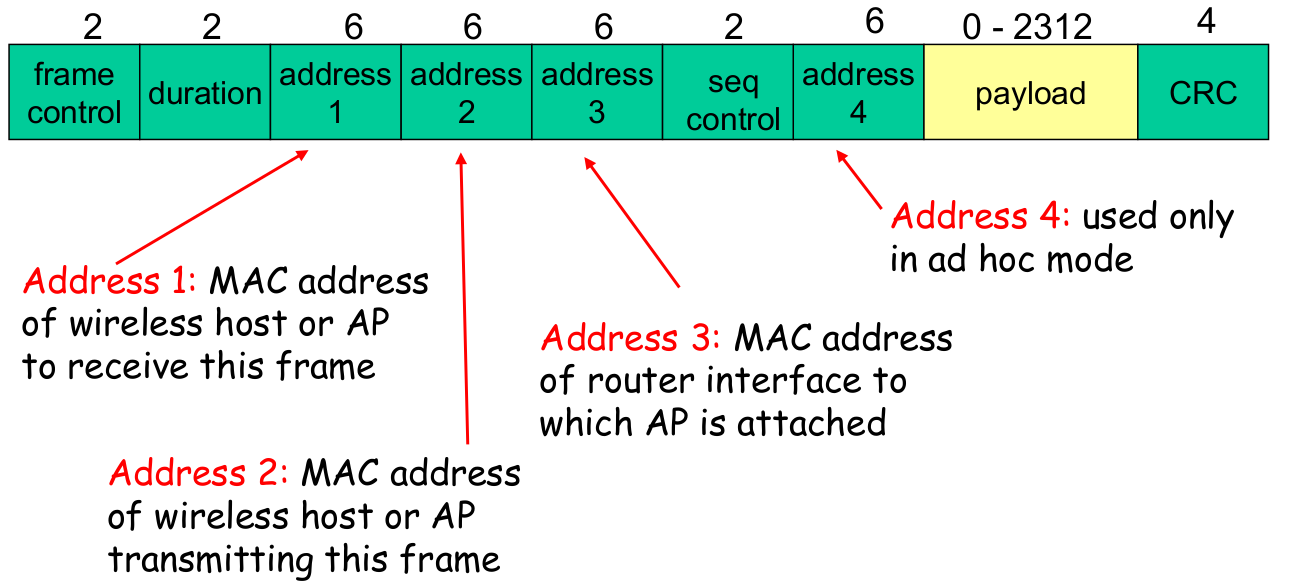
\includegraphics[width=0.48\textwidth]{802_11_addr}
  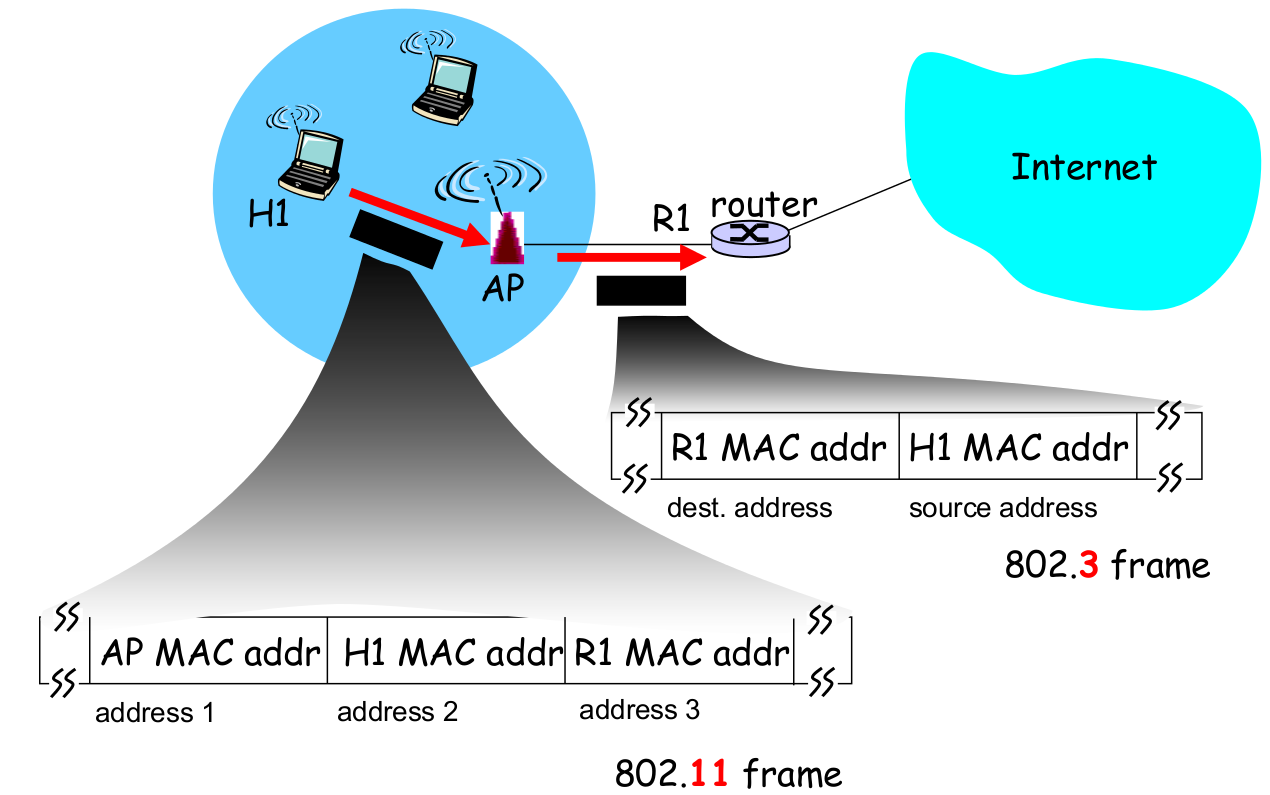
\includegraphics[width=0.48\textwidth]{802_11_addr2}
\end{figure}

\key{802.11: advanced capabilities}
\begin{figure}[H]
  \centering
  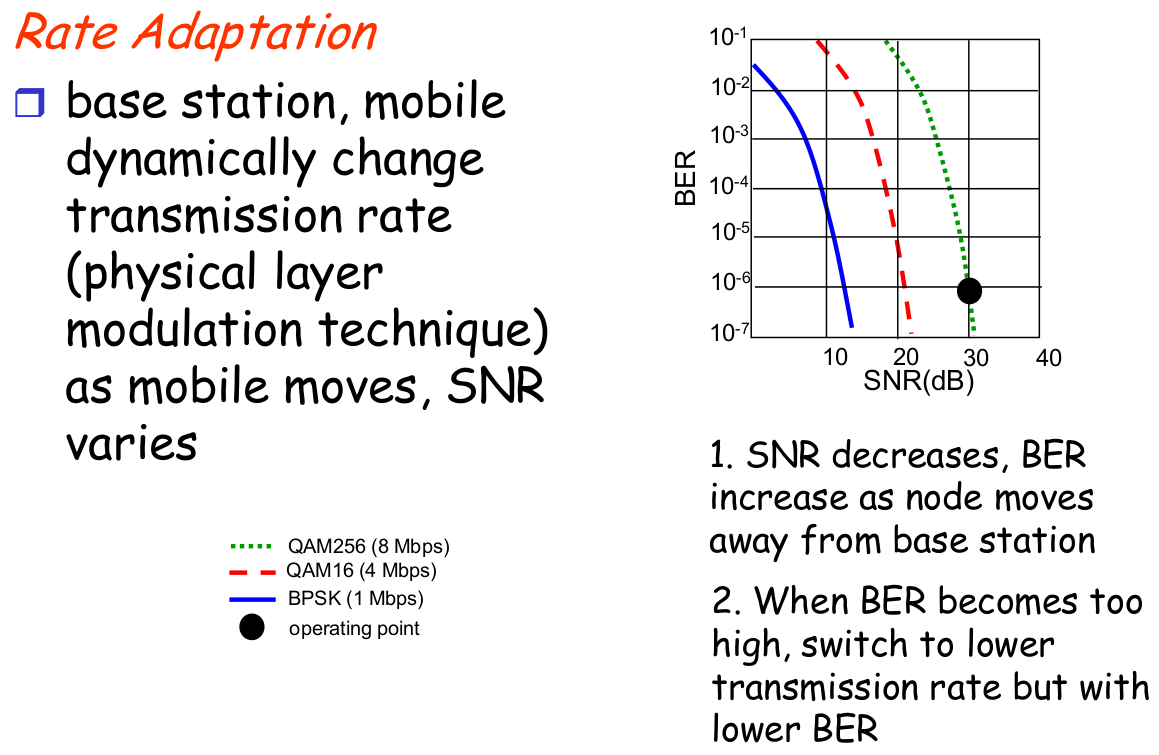
\includegraphics[width=0.48\textwidth]{802_11_adv}
  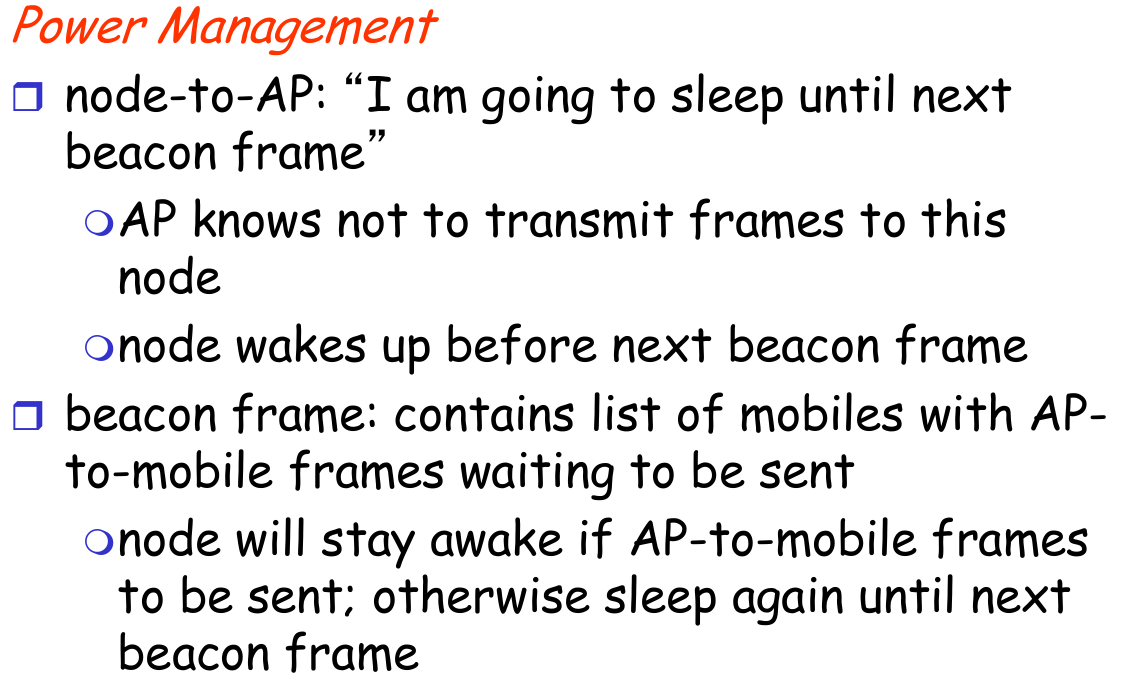
\includegraphics[width=0.48\textwidth]{802_11_adv2}
\end{figure}

\subsection{Cellular Internet Access}

\subsection{Principles: addressing and routing to mobile users}

\subsection{Mobile IP}

\key{GSM: handoff with common MSC}
\begin{figure}[H]
  \centering
  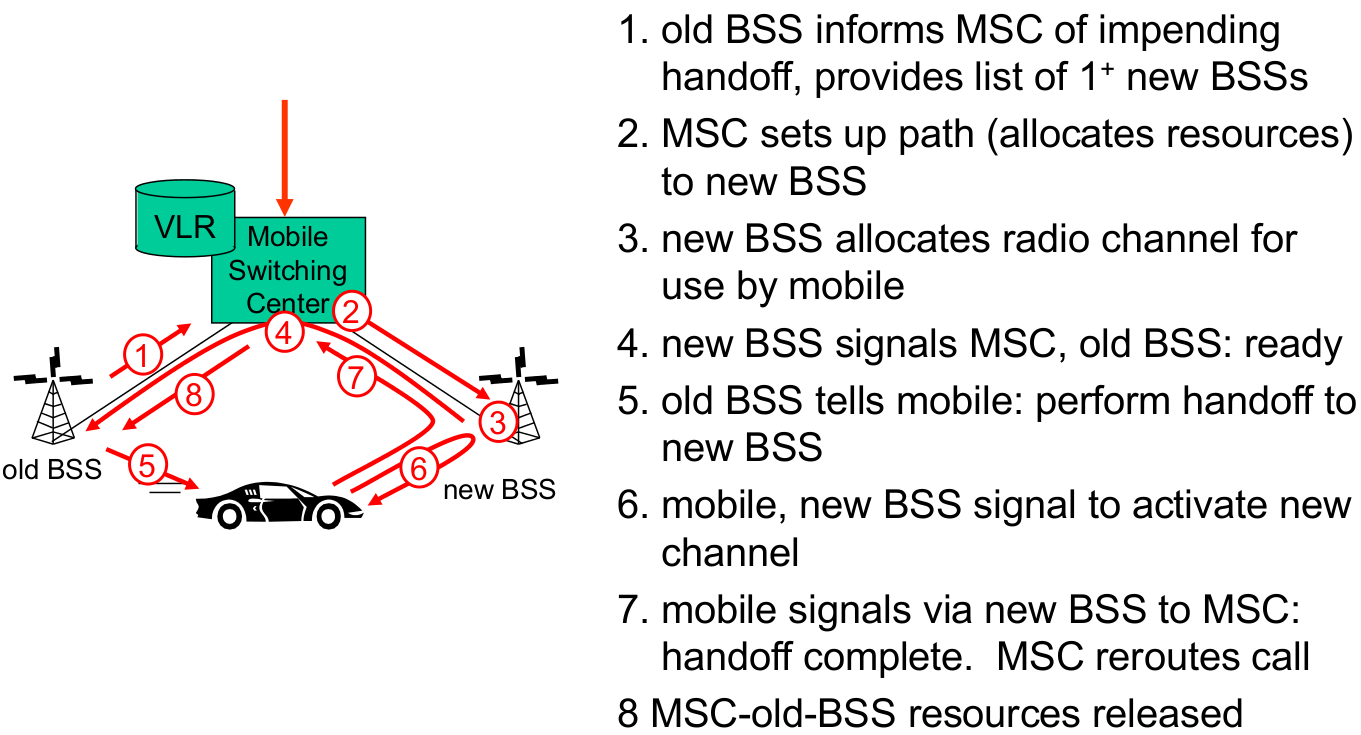
\includegraphics[width=0.48\textwidth]{gsm_handoff}
\end{figure}



\key{Mobility: GSM versus Mobile IP}
\begin{figure}[H]
  \centering
  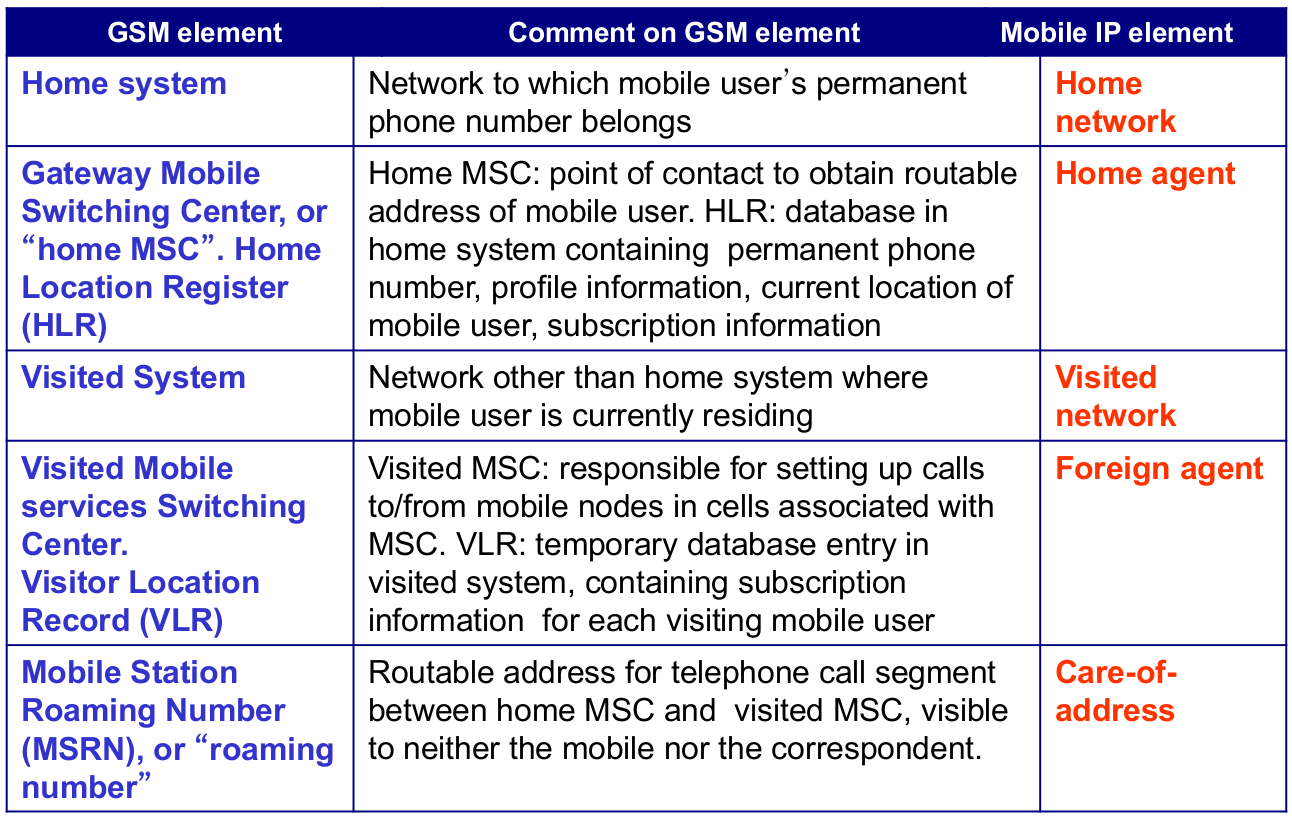
\includegraphics[width=0.48\textwidth]{gsm_vs_mobileip}
\end{figure}





